\question[6] (8分)某同学描绘一种电子元件的$I-U$关系图象,采用的实验电路图如图1所示,\circled{V}  为电压表,\circled{\small{mA}} 为电流表,E为电源(电动势约6V),R为滑动变阻器(最大阻值$20\Omega$,$R_0$为定值电阻,S为开关。\begin{center}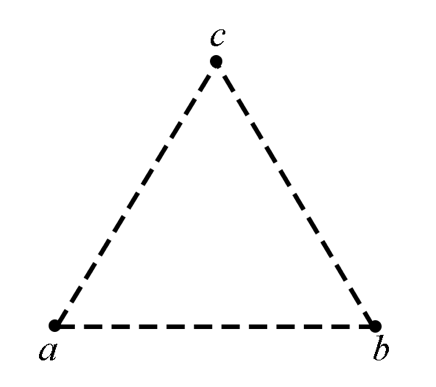
\includegraphics[width=12cm]{img/image11.png}\end{center}

(1)请用笔画线代替导线,将图2所示的实物电路连接完整。

(2)调节滑动变阻器,记录电压表和电流表的示数如表:
\begin{table}[h]
    \begin{center}
        \begin{tabular}{|l|l|l|l|l|l|l|l|}
            \hline
            电压U/V  & 0.000 & 0.250 & 0.500 & 0.650 & 0.700 & 0.725 & 0.750 \\ \hline
            电流I/mA & 0.00  & 0.10  & 0.25  & 0.60  & 1.70  & 4.30  & 7.50  \\ \hline
            \end{tabular}
    \end{center}
\end{table}

请根据表中的数据,在方格纸上作出该元件的$I-U$图线。

(3)根据作出的$I-U$图线可知,该元件是\key{非线性}(选填“线性”或“非线性”)元件。

(4)在上述测量中,如果用导线代替电路中的定值电阻$R_0$,会导致的两个后果是\key{BC}。

(A)电压和电流的测量误差增大

(B)可能因电流过大烧坏待测元件

(C)滑动变阻器允许的调节范围变小

(D)待测元件两端电压的可调节范围变小

\newpage
\question[6] (10分)疫情期间“停课不停学”,小明同学在家自主开展实验探究。用手机拍摄物体自由下落的视频,得到分帧图片,利用图片中小球的位置来测量当地的重力加速度,实验装置如图1所示。

(1)家中有乒乓球、小塑料球和小钢球,其中最适合用作实验中下落物体的是\key{小钢球}。

(2)下列主要操作步骤的正确顺序是\key{①③④②}。(填写各步骤前的序号)①把刻度尺竖直固定在墙上②捏住小球,从刻度尺旁静止释放③手机固定在三角架上,调整好手机镜头的位置④打开手机摄像功能,开始摄像

(3)停止摄像,从视频中截取三帧图片,图片中的小球和刻度如图2所示。已知所截取的图片相邻两帧之间的时间间隔为$\frac{1}{6}s$,刻度尺的分度值是$1mm$,由此测得重力加速度为\key{9.6(9.5$\sim$9.7)}$m/s^{2}$。

(4)在某次实验中,小明释放小球时手稍有晃动,视频显示小球下落时偏离了竖直方向。从该视频中截取图片,\key{仍能}(选填“仍能”或“不能”)用

(3)问中的方法测出重力加速度。\begin{center}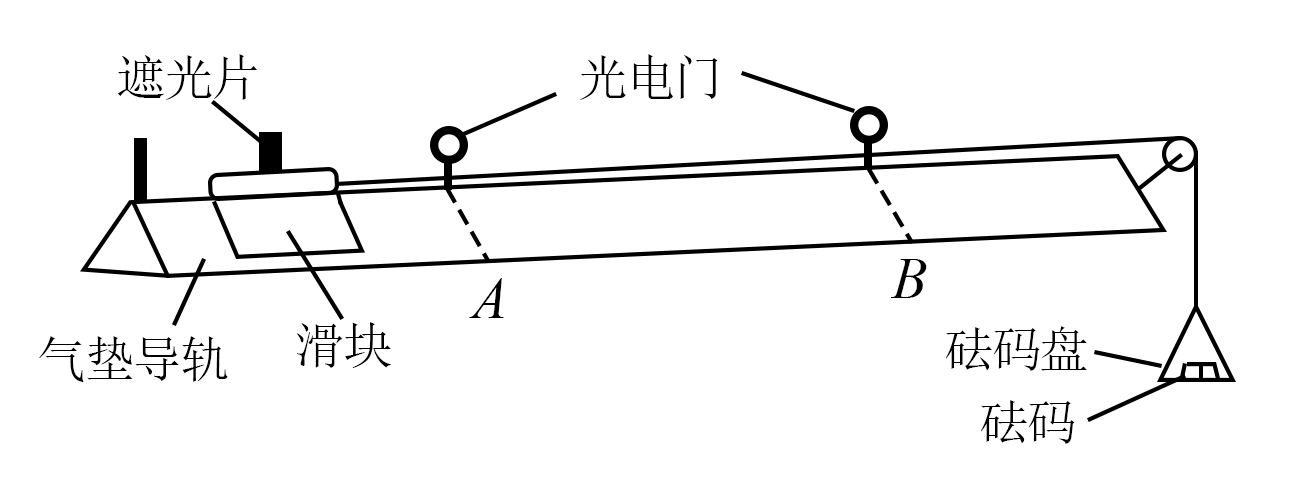
\includegraphics[]{img/image12.png}\end{center}

\newpage
\textbf{[选修3-5](12分)}
\question[6] (3分)“测温枪”(学名“红外线辐射测温仪”)具有响应快、非接触和操作方便等优点。它是根据黑体辐射规律设计出来的,能将接收到的人体热辐射转换成温度显示。若人体温度升高,则人体热辐射强度I及其极大值对应的波长$\lambda$的变化情况是\key{仍能}

A.I增大,$\lambda$增大

B.I增大,$\lambda$减小	

C.I减小,$\lambda$增大	

D.I减小,$\lambda$减小

\question[6] (4分)大量处于某激发态的氢原子辐射出多条谱线,其中最长和最短波长分别为$\lambda_{1}$和$\lambda_{2}$,则该激发态与基态的能量差为\key{$\frac{h c}{\lambda_{2}}$},波长为$\lambda_{1}$的光子的动量为\key{$\frac{h}{\lambda_{1}}$}。(已知普朗克常量为h,光速为c)
\question[6] (5分)一只质量为$1.4kg$的乌贼吸入$0.1kg$的水,静止在水中。遇到危险时,它在极短时间内把吸入的水向后全部喷出,以$2m/s$的速度向前逃窜。求该乌贼喷出的水的速度大小v。
\begin{solution}{4cm}
    $v=28m/s$
\end{solution}
\textbf{【选做题】本题包括A、B两小题,请选定其中一小题,并在相应的答题区域内作答。若多做,则按A小题评分。A.[选修3-3](12分)}
\question[6] (3分)玻璃的出现和使用在人类生活里已有四千多年的历史,它是一种非晶体。下列关于玻璃的说法正确的有\key{AC}

A.没有固定的熔点

B.天然具有规则的几何形状	

C.沿不同方向的导热性能相同

D.分子在空间上周期性排列
\question[6] (4分)一瓶酒精用了一些后,把瓶盖拧紧,不久瓶内液面上方形成了酒精的饱和汽,此时\key{有}(选填“有”或“没有”)酒精分子从液面飞出。当温度升高时,瓶中酒精饱和汽的密度\key{增大}(选填“增大”“减小”或“不变”)。
\question[6] (5分)一定质量的理想气体从状态A经状态B变化到状态C,其$p-\frac{1}{V}$图象如图所示,求该过程中气体吸收的热量Q。\begin{center}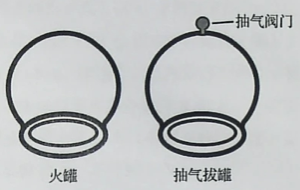
\includegraphics[width=4cm]{img/image13.png}\end{center}
\begin{solution}{4cm}
    $Q=2\times 10^5J$
\end{solution}

\newpage
\textbf{B.[选修3-4](12分)}
\question[6] 电磁波广泛应用在现代医疗中。下列属于电磁波应用的医用器械有\key{A}

A.杀菌用的紫外灯

B.拍胸片的X光机

C.治疗咽喉炎的超声波雾化器

D.检查血流情况的“彩超”机
\question[6] 我国的光纤通信技术处于世界领先水平。光纤内芯(内层玻璃)的折射率比外套(外层玻璃)的\key{大}(选填“大”或“小”)。某种光纤的内芯在空气中全反射的临界角为$43^\prime$,则该内芯的折射率为\key{1.5}。(取$\sin43^{\circ}=0.68$,$\cos43^{\circ}=0.73$,结果保留2位有效数字)

\question[6] 国际宇航联合会将$2020$年度“世界航天奖”授予我国“嫦娥四号”任务团队。“嫦娥四号”任务创造了多项世界第一。在探月任务中,“玉兔二号”月球车朝正下方发射一束频率为f的电磁波,该电磁波分别在月壤层的上、下表面被反射回来,反射波回到“玉兔二号”的时间差为$△t.$已知电磁波在月壤层中传播的波长为$\lambda$,求该月壤层的厚度d。
\begin{solution}{4cm}
    $d=\frac{1}{2} \lambda f \Delta t$
\end{solution}

\end{questions}
\group{计算题}{本题共3小题,共计47分。解答时请写出必要的文字说明、方程式和重要的演算步骤。只写出最后答案的不能得分。有数值计算的题,答案中必须明确写出数值和单位。}
\begin{questions}[p]
\question[6] (15分)如图所示,电阻为$0.1\Omega$的正方形单匝线圈$abcd$的边长为$0.2m$,bc边与匀强磁场边缘重合。磁场的宽度等于线圈的边长,磁感应强度大小为$0.5T.$在水平拉力作用下,线圈以$8m/s$的速度向右穿过磁场区域。求线圈在上述过程中

(1)感应电动势的大小E;

(2)所受拉力的大小F;

(3)感应电流产生的热量Q。\begin{center}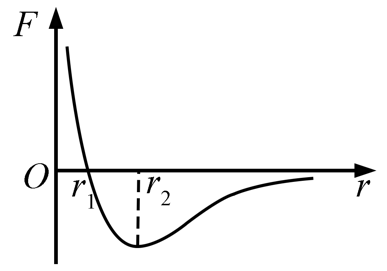
\includegraphics[]{img/image14.png}\end{center}
\begin{solution}{4cm}
    (1)感应电动势的大小为0.8V

    (2)所受拉力的大小为0.8N

    (3)感应电流产生的热量为0.32J
\end{solution}

\newpage
\question[6] (16分)如图所示,鼓形轮的半径为R,可绕固定的光滑水平轴O转动。在轮上沿相互垂直的直径方向固定四根直杆,杆上分别固定有质量为m的小球,球与O的距离均为2R。在轮上绕有长绳,绳上悬挂着质量为M的重物。重物由静止下落,带动鼓形轮转动。重物落地后鼓形轮匀速转动,转动的角速度为$\omega$。绳与轮之间无相对滑动,忽略鼓形轮、直杆和长绳的质量,不计空气阻力,重力加速度为g。求:

(1)重物落地后,小球线速度的大小v;

(2)重物落地后一小球转到水平位置A,此时该球受到杆的作用力的大小F;

(3)重物下落的高度h。\begin{center}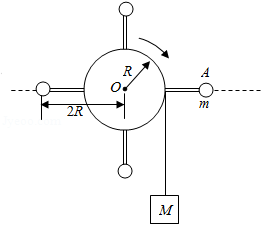
\includegraphics[]{img/image15.png}\end{center}
\begin{solution}{4cm}
    (1)重物落地后,小球线速度的大小为$2R\omega$

    (2)重物落地后一小球转到水平位置A,此时该球受到杆的作用力的大小为$m \sqrt{4 R^{2} \omega^{4}+g^{2}}$

    (3)重物下落的高度为$\frac{M+16 m}{2 M g}(\omega R)^{2}$
\end{solution}
\newpage
\question[6] (16分)空间存在两个垂直于$Oxy$平面的匀强磁场,y轴为两磁场的边界,磁感应强度分别为$2B_{0}$、$3B_{0}.$甲、乙两种比荷不同的粒子同时从原点O沿x轴正向射入磁场,速度均为v。甲第1次、第2次经过y轴的位置分别为P、Q,其轨迹如图所示。甲经过Q时,乙也恰好同时经过该点。已知甲的质量为m,电荷量为q。不考虑粒子间的相互作用和重力影响。求:

(1)Q到O的距离d;

(2)甲两次经过P点的时间间隔△t。

(3)乙的比荷$\frac{q^{\prime}}{m^{\prime}}$可能的最小值。\begin{center}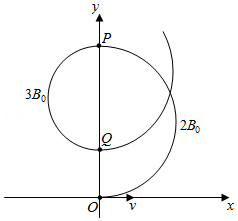
\includegraphics[]{img/image16.png}\end{center}
\begin{solution}{4cm}
    (1)$d=\frac{m v}{3 q B_{0}}$

    (2)$\Delta t=\frac{2 \pi m}{q B_{0}}$

    (3)$\frac{q^{\prime}}{m^{\prime}}_{min}=\frac{2 q}{m}$
\end{solution}